% ============================================================
%  SE2RoadNet pipeline -- standalone TikZ figure for slides.
%  Mirrors paper/present/fig_arch.tex but for the SE(2)-Equivariant variant.
%  Compile once: pdflatex fig_arch_se2.tex   ->   fig_arch_se2.pdf
% ============================================================
\documentclass[tikz,border=8pt]{standalone}
\usepackage{lmodern}
\usepackage{amsmath, amssymb}
\usepackage[T1]{fontenc}
\usepackage{xcolor}
\usetikzlibrary{positioning, fit, backgrounds, arrows.meta}

\definecolor{alertred}{HTML}{C0392B}

\begin{document}
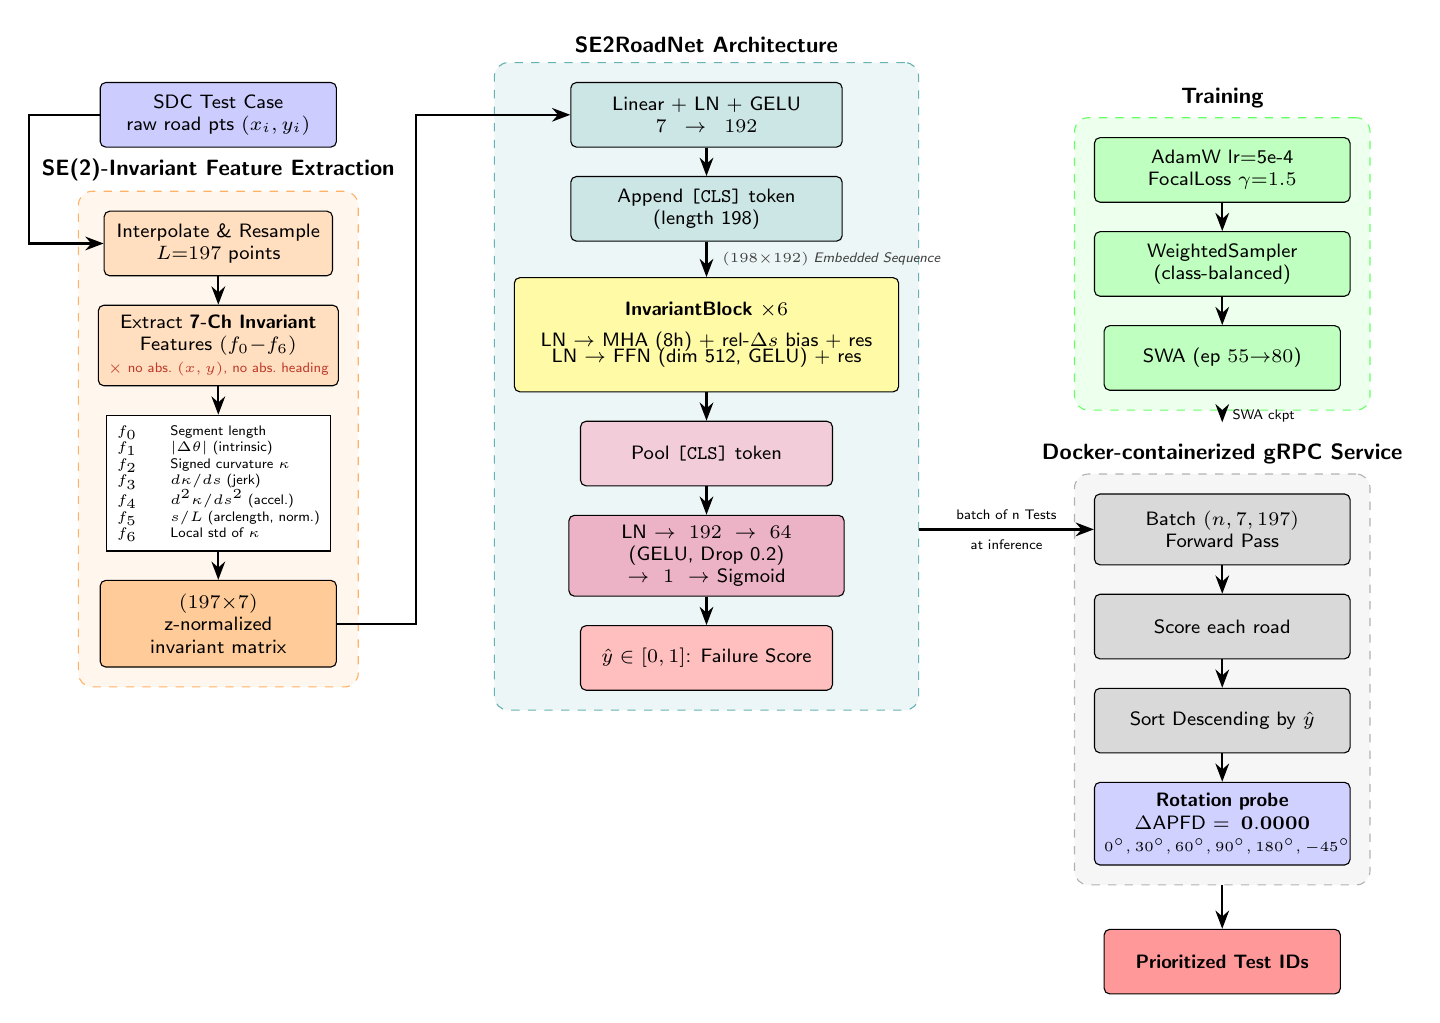
\begin{tikzpicture}[
  font=\sffamily\scriptsize,
  >=Stealth,
  node distance=0.36cm,
  arr/.style={->, thick},
  blk/.style={draw, rounded corners=2pt, fill=#1, align=center,
              inner sep=3.5pt, minimum width=2.9cm, minimum height=0.82cm},
  grp/.style={draw=#1!60, dashed, rounded corners=5pt,
              inner sep=7pt, fill=#1!7},
  htitle/.style={font=\sffamily\bfseries\footnotesize},
]

%% ===== LEFT: INPUT & SE(2)-INVARIANT FEATURE EXTRACTION =====

\node[blk=blue!20, minimum width=3.0cm] (sdc) at (0,0)
    {SDC Test Case\\raw road pts $(x_i, y_i)$};

\node[blk=orange!25, below=0.80cm of sdc] (resamp)
    {Interpolate \& Resample\\$L{=}197$ points};

\node[blk=orange!25, below=0.36cm of resamp, minimum height=1.0cm] (feat)
    {Extract \textbf{7-Ch Invariant}\\Features $(f_0{-}f_6)$\\
     \textcolor{alertred}{\tiny $\times$ no abs.\ $(x,y)$, no abs.\ heading}};

\node[draw, fill=white, inner sep=3pt, below=0.36cm of feat,
      font=\sffamily\tiny, minimum width=2.85cm] (ftab)
    {\begin{tabular}{@{}ll@{}}
       $f_0$ & Segment length \\
       $f_1$ & $|\Delta\theta|$ (intrinsic) \\
       $f_2$ & Signed curvature $\kappa$ \\
       $f_3$ & $d\kappa/ds$ (jerk) \\
       $f_4$ & $d^2\kappa/ds^2$ (accel.) \\
       $f_5$ & $s/L$ (arclength, norm.) \\
       $f_6$ & Local std of $\kappa$ \\
     \end{tabular}};

\node[blk=orange!40, below=0.36cm of ftab, minimum width=3.0cm,
      minimum height=1.1cm] (znorm)
    {$(197{\times}7)$\\z-normalized\\invariant matrix};

\begin{pgfonlayer}{background}
  \node[grp=orange, fit=(resamp)(feat)(ftab)(znorm),
        label={[htitle]above=2pt:SE(2)-Invariant Feature Extraction}] (leftgrp) {};
\end{pgfonlayer}

%% ===== MIDDLE: SE2ROADNET ARCHITECTURE =====

\node[blk=teal!20, minimum width=3.2cm, text width=3.2cm] (proj) at (6.2,0)
    {Linear + LN + GELU\\$7 \to 192$};

\node[blk=teal!20, minimum width=3.2cm, text width=3.2cm, below=0.36cm of proj] (cls)
    {Append \texttt{[CLS]} token\\(length 198)};

\node[blk=yellow!35, minimum width=3.3cm, minimum height=1.45cm,
      below=0.45cm of cls] (enc)
    {\begin{tabular}{c}
      \textbf{InvariantBlock $\times 6$}\\[3pt]
      {\scriptsize LN $\rightarrow$ MHA (8h) + rel-$\Delta s$ bias + res}\\[-2pt]
      {\scriptsize LN $\rightarrow$ FFN (dim 512, GELU) + res}
    \end{tabular}};

\node[blk=purple!20, minimum width=3.2cm, below=0.36cm of enc] (pool)
    {Pool \texttt{[CLS]} token};

\node[blk=purple!30, minimum width=3.2cm, text width=3.25cm,
      below=0.36cm of pool, minimum height=0.95cm] (mlp)
    {LN $\to 192 \to 64$\\(GELU, Drop 0.2)\\$\to 1 \to$ Sigmoid};

\node[blk=red!25, minimum width=3.2cm, below=0.36cm of mlp] (yhat)
    {$\hat{y} \in [0,1]$: Failure Score};

\begin{pgfonlayer}{background}
  \node[grp=teal,
        fit=(proj)(cls)(enc)(pool)(mlp)(yhat),
        label={[htitle]above:SE2RoadNet Architecture}] (midgrp) {};
\end{pgfonlayer}

%% ===== RIGHT-TOP: TRAINING =====

\node[blk=green!25, minimum width=3.0cm, text width=3.0cm] (adam) at (12.75, -0.7)
    {AdamW lr$=$5e-4\\FocalLoss $\gamma{=}1.5$};

\node[blk=green!25, minimum width=3.0cm, text width=3.0cm,
      below=0.36cm of adam] (sampler)
    {WeightedSampler\\(class-balanced)};

\node[blk=green!25, minimum width=3.0cm, below=0.36cm of sampler] (swabox)
    {SWA (ep $55{\to}80$)};

\begin{pgfonlayer}{background}
  \node[grp=green, fit=(adam)(sampler)(swabox),
        label={[htitle]above:Training}] (swagrp) {};
\end{pgfonlayer}

%% ===== RIGHT-BOTTOM: DOCKER + INFERENCE =====

\node[blk=gray!30, minimum width=3.0cm, text width=3.0cm,
      below=1.05cm of swagrp.south, minimum height=0.90cm] (bfwd)
    {Batch $(n,7,197)$\\Forward Pass};

\node[blk=gray!30, minimum width=3.0cm, text width=3.0cm,
      below=0.36cm of bfwd, minimum height=0.82cm] (scorerd)
    {Score each road};

\node[blk=gray!30, minimum width=3.0cm, text width=3.0cm,
      below=0.36cm of scorerd, minimum height=0.82cm] (sortd)
    {Sort Descending by $\hat{y}$};

\node[blk=blue!18, minimum width=3.0cm, text width=3.0cm,
      below=0.36cm of sortd, minimum height=1.05cm] (rotprobe)
    {\textbf{Rotation probe}\\$\Delta$APFD $= \mathbf{0.0000}$\\
     {\tiny $0^\circ, 30^\circ, 60^\circ, 90^\circ, 180^\circ, {-}45^\circ$}};

\begin{pgfonlayer}{background}
  \node[grp=gray, fit=(bfwd)(scorerd)(sortd)(rotprobe),
        label={[htitle]above:Docker-containerized gRPC Service}] (dkgrp) {};
\end{pgfonlayer}

\node[blk=red!40, minimum width=3.0cm, below=0.55cm of dkgrp.south] (result)
    {\textbf{Prioritized Test IDs}};

%% ===== ARROWS =====

\draw[arr] (sdc.west) -- ++(-0.9,0) |- (resamp.west);
\draw[arr] (resamp) -- (feat);
\draw[arr] (feat)   -- (ftab);
\draw[arr] (ftab)   -- (znorm);

\draw[arr] (znorm.east) -- ++(1.00,0) |- (proj.west);

\draw[arr] (proj) -- (cls);
\draw[arr] (cls)  -- node[midway, right=2pt, font=\sffamily\tiny\itshape, text=black!75]
    {$(198{\times}192)$ Embedded Sequence} (enc);
\draw[arr] (enc)  -- (pool);
\draw[arr] (pool) -- (mlp);
\draw[arr] (mlp)  -- (yhat);

\coordinate (dktitle) at ([yshift=0.65cm]dkgrp.north);
\draw[arr] (adam.south) -- (sampler.north);
\draw[arr] (sampler.south) -- (swabox.north);
\draw[arr] (swagrp.south) -- node[midway, right, font=\sffamily\tiny] {SWA ckpt} (dktitle);
\draw[arr] (bfwd)    -- (scorerd);
\draw[arr] (scorerd) -- (sortd);
\draw[arr] (sortd)   -- (rotprobe);
\draw[arr] (dkgrp.south) -- (result);

\draw[arr] (midgrp.east |- bfwd.west) -- (bfwd.west)
    node[midway, above, font=\sffamily\tiny] {batch of n Tests}
    node[midway, below, font=\sffamily\tiny] {at inference};

\end{tikzpicture}
\end{document}
